\chapter{Measurement Methodology}

This chapter is dedicated to answering the questions of what was measured and how results were obtained. Firstly, the measurement setup is discussed in view of the necessity to verify the recorded data. Subsequently,  the GNU Radio flowgraphs are explained. Secondly, with reference to the flowgraphs measurement metrics are formally defined.  Lastly, an overview of the semi-automatic measurement script system designed to automate, therefore accelerate the process of file system management, data processing and result plotting is given.

\section{Measurement Setup}

The setup consists of two USRP2s from Ettus Research and two USRP 2920s from National Instruments. Where the former pair is programmed as receiver and sniffer and the latter  as senders as depicted in \ref{fig:measurement-setup}. Each USRP was connected to a gigabit switch through a LAN cabel. The scripts running on the devices were launched from the institute's computer with the IP 134.130.223.151, which was remote controlled from my private laptop. Table \ref{tab:measurement-parameters} and figure \ref{fig:measurement-setup}  contain all other necessary information to reproduce the measurement results.

\begin{figure}[tb]
	\label{fig:measurement-setup}
	\begin{center}
		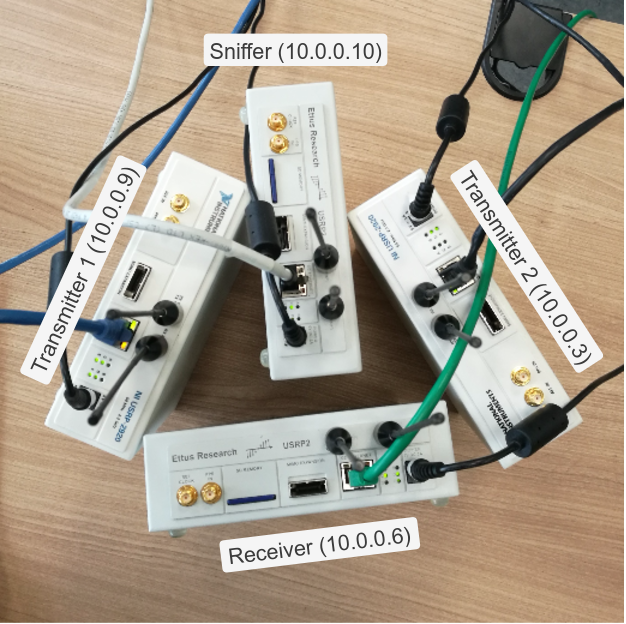
\includegraphics[width=0.5\textwidth]{pictures/measurement_setup}
	\end{center}
	\caption{Photo of the measurement setup}
\end{figure}

% Measurement parameters
\begin{table}
	\label{tab:measurement-parameters}
	\begin{center}
		\begin{tabular}{p{3.5cm}p{10cm}}
			\toprule
			a & b \\
			c & d \\
			\bottomrule	
		\end{tabular}\caption{Setup parameters}
	\end{center}
\end{table}


\section{GNU Radio Flowgraphs}

%\subsection{Common Variables}
%
%Our GNU Radio pure ALOHA and non-persistent/1-persistent CSMA implementations are placed on top of a common PHY layer warranting comparability. The specific PHY layer implementation is beyond this work's scope, but a few parameters common to all flowgraphs shall be discussed nonetheless. Hereinafter, these variables and their values will not be mentioned unless they are important concerning the interpretation of results.
%
%\begin{figure}[ht]
%	\label{fig:grc-common-variables}
%	\begin{center}
%		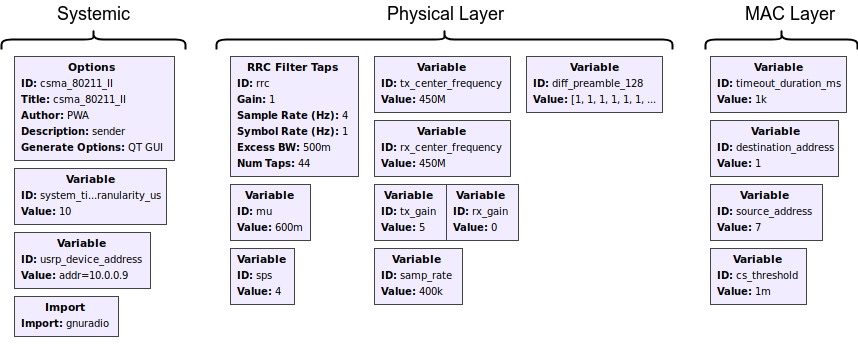
\includegraphics[width=\textwidth]{pictures/grc_common_variables}
%	\end{center}
%\caption{Variables Common to All Flowgraphs}
%\end{figure}     

\subsection{Receiver and Sniffer}

Figure \ref{fig:grc-receiver} shows the two-way handshake receiving logic. After frame integrity is checked and type is confirmed to be data frame an acknowledgment is generated. The frame probe blocks record the times when the frames reach certain positions in the flowgraph representing the occurrence of events such as frame reception, passed or failed frame integrity check and more. Note that the address check is disabled so that the receiver may receive frames from any sender.

The sniffer consists only of a single frame probe block, which records detected power above noise level during the whole measurement. The sniffer provides valuable insight of what is actually going on in the channel from a "neutral" point of view. Neutral in the sense of:

\begin{itemize}
	\item A clear distinction between the senders can be made according to the energy levels, since the sniffer is located between the senders and transmission gains were set accordingly.
	\item Sensing the channel is possible during the whole measurement time, because the sniffer is never sending.
\end{itemize}

In a nutshell, the sniffer is a valuable debugging and verification tool as described in more detail in section \ref{sec:measurement-metrics}.

\begin{sidewaysfigure}[ht]
	\label{fig:grc-receiver}
	\begin{center}
		\subfloat[Receiver]{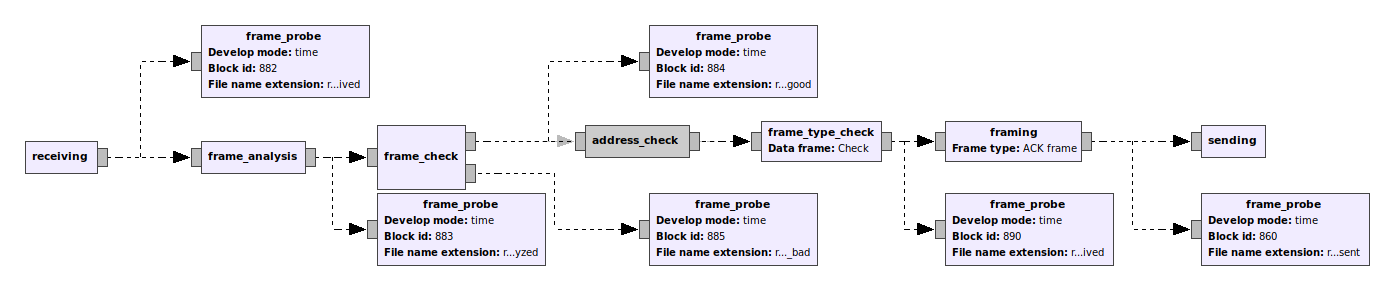
\includegraphics[width=\textwidth]{pictures/grc_receiver_flowgraph}}
		\vskip 40pt
		\subfloat[Sniffer]{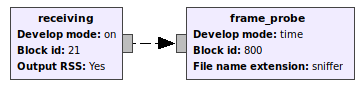
\includegraphics[width=0.3\textwidth]{pictures/grc_sniffer_flowgraph}}
	\end{center}
	\caption{GRC Receiver Flowgraphs}
\end{sidewaysfigure}

\subsection{Pure ALOHA Transmitter}

\begin{sidewaysfigure}[h]
	\label{fig:grc-aloha-sender}
	\begin{center}
		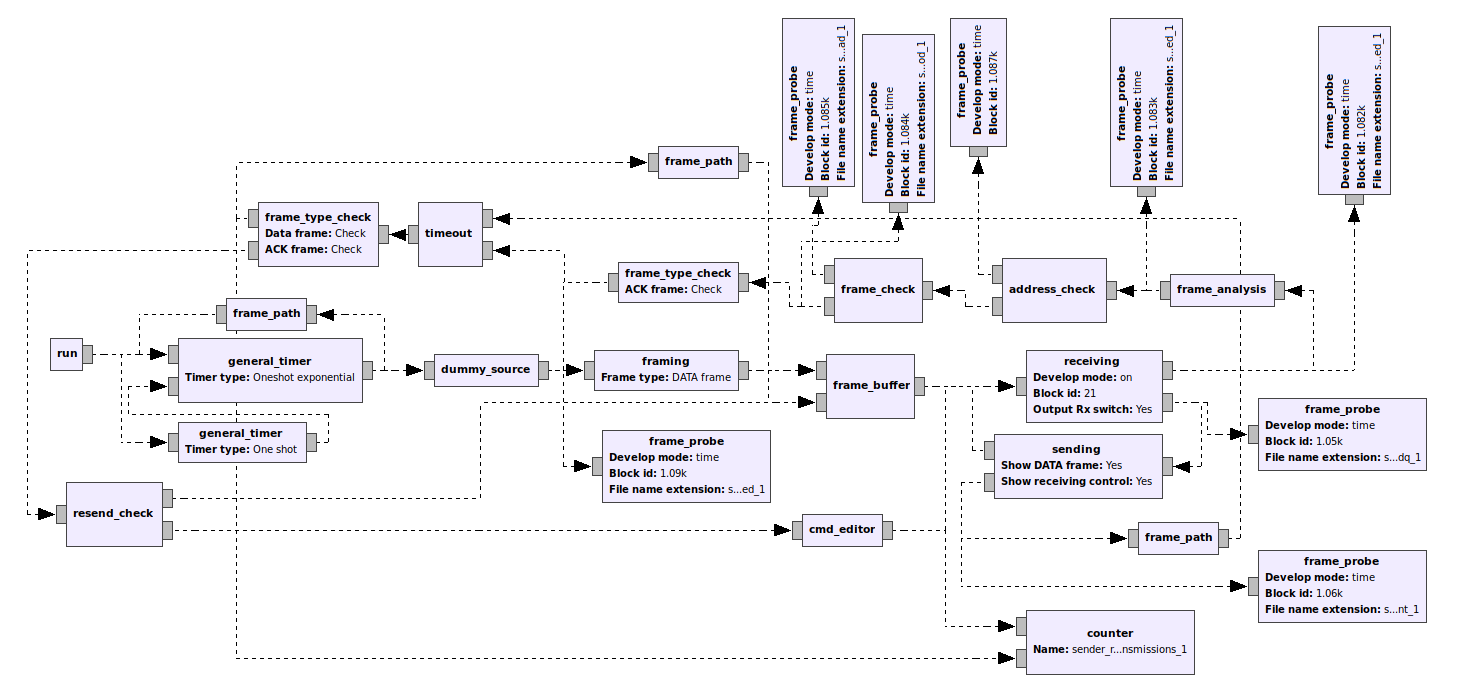
\includegraphics[width=\textwidth]{pictures/grc_aloha_transmitter_flowgraph}
\end{center}
\caption{GRC Pure ALOHA Transmitter Flowgraph}
\end{sidewaysfigure}

\subsection{CSMA Transmitter}

\begin{sidewaysfigure}[h]
	\label{fig:grc-csma-sender}
	\begin{center}
		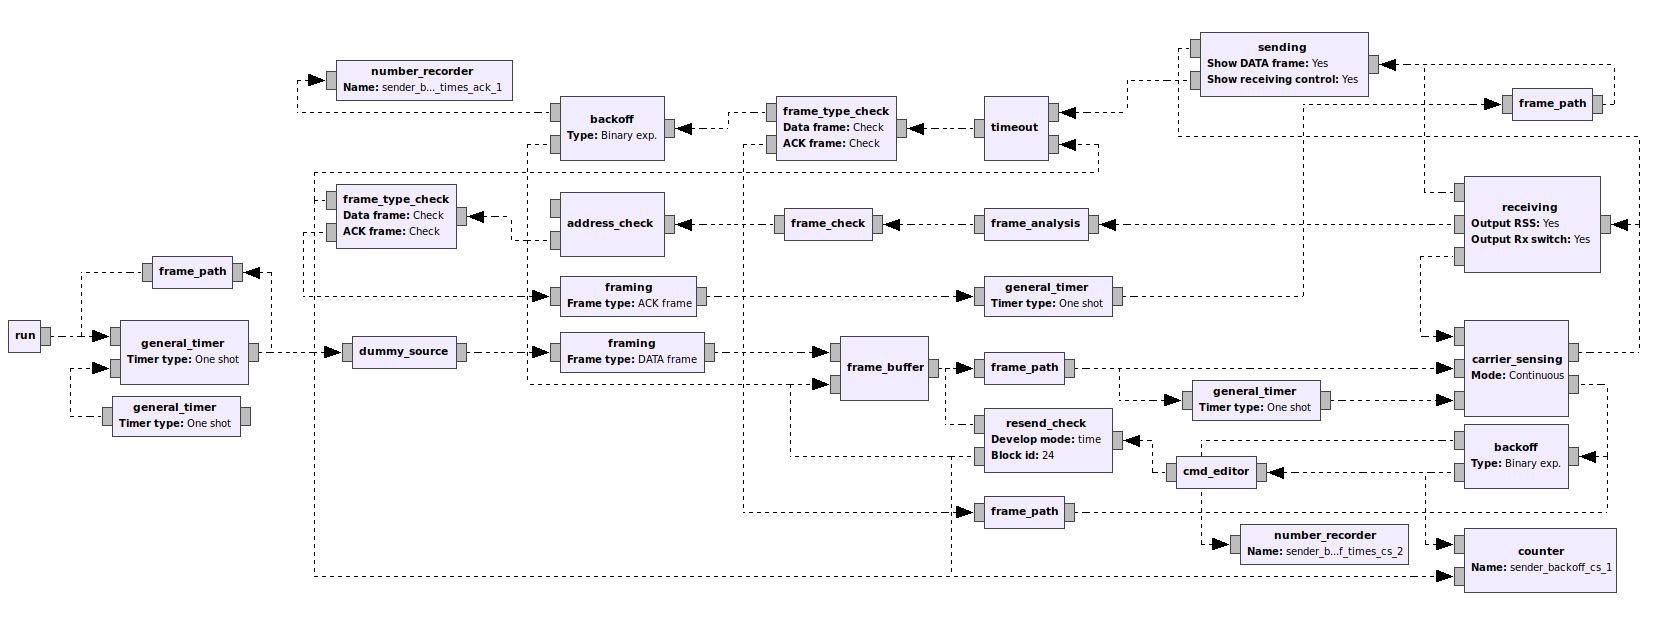
\includegraphics[width=\textwidth]{pictures/grc_csma_transmitter_flowgraph}
\end{center}
\caption{GRC CSMA Transmitter Flowgraph}
\end{sidewaysfigure}

\clearpage

\section{Measurement Metrics}
\label{sec:measurement-metrics}

\section{Measurement Script System}
\label{sec:script-system}

\begin{figure}[ht]
	\label{fig:script-system}
	\begin{center}
		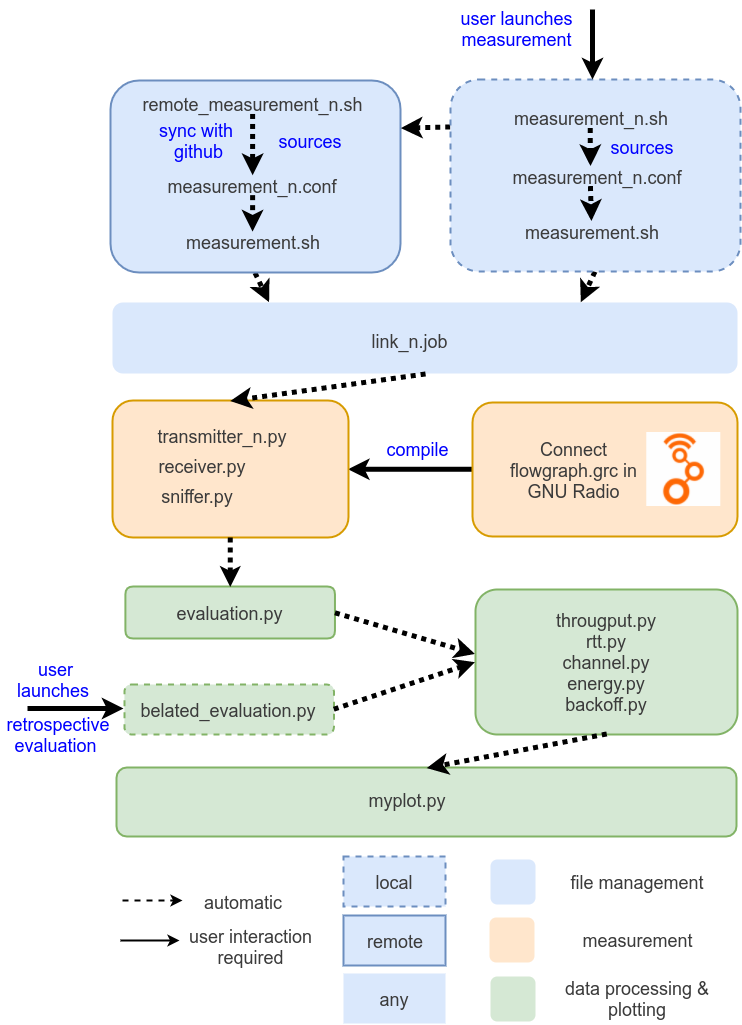
\includegraphics[width=0.6\textwidth]{pictures/script_system}
	\end{center}
	\caption{The Three-Phase Measurement Script System}
\end{figure}